%~~~~~~~~~~~~~~~~~~~~~~~~~~~~~~~~~~~~~~~~~~~~~~~~~~~~~~~~~~~~~~~~~~~~~~~~~~~~~~~~~~~~~~~~~%
% IISER Thiruvananthapuram Beamer Presentation Template
% Author: Nikhil Alex Verghese, BS-MS '17
%
% Licensed under Creative Commons Attribution–NonCommercial–ShareAlike 4.0
% (CC BY-NC-SA 4.0). More info: https://creativecommons.org/licenses/by-nc-sa/4.0/
%
% Suggestions/Feedback: nikhil.alexv17@alumni.iisertvm.ac.in
%~~~~~~~~~~~~~~~~~~~~~~~~~~~~~~~~~~~~~~~~~~~~~~~~~~~~~~~~~~~~~~~~~~~~~~~~~~~~~~~~~~~~~~~~~%

% Comments like this begin with a % character. 
% Ctrl+b for \textbf{bold} and Ctrl+i for \textit{italics} 
% Ctrl+/ to comment out lines

% Refer to these links for useful beamer tips and tricks
% http://tug.ctan.org/macros/latex/contrib/beamer/doc/beameruserguide.pdf
% https://www.overleaf.com/learn/latex/Beamer
% https://en.wikipedia.org/wiki/Beamer_%28LaTeX%29 --> `External Links'

%=========================================================================================
% PREAMBLE (PACKAGES AND DOCUMENT CONFIGURATION)
%=========================================================================================
\documentclass[10pt,presentation,shownotes,aspectratio=169]{beamer}
% Add in 'draft' to parameters above to halt graphics and TikZ and decrease compile time

% Load configuration files
\input{Configuration/Preamble}     % Packages, custom frame and block styles
\input{Configuration/MathLetters}  % Math symbols and alphabet macros
% Set custom colours here:

\definecolor{mygrey}{RGB}{173,173,173}      % Color definitions

%=========================================================================================
% INTRODUCTORY PAGES
%=========================================================================================
% Custom input fields are marked with [] in the intro sections. 
% Rewrite inputs according to capitalisation within brackets (First Letter Capital/ALL UPPERCASE/all small letters). 
% Go through each intro page and update all of your personal information accordingly. 
% Read all uncommented lines carefully.
%~~~~~~~~~~~~~~~~~~~~~~~~~~~~~~~~~~~~~~~~~~~~~~~~~~~~~~~~~~~~~~~~~~~~~~~~~~~~~~~~~~~~~~~~~%

% \title[\color{white} LWC
% \hspace{0.3cm}\insertframenumber/\inserttotalframenumber]{\LARGE Mischief in the Cube: A Study of the Saturnin}
% \author[Kriti Arora, 12240880]{Kriti Arora [4pt] 12240880}
% \institute[IIT Bhilai]{IIT Bhilai}

\title{Mischief in the Cube: A Study of the Saturnin}
\author[Kriti Arora, 12240880]{Kriti Arora 12240880}
\institute[IIT Bhilai]{IIT Bhilai}


% \title[\color{white} Short Pres. Title
% \hspace{0.3cm}\insertframenumber/\inserttotalframenumber]{\LARGE [Extended Presentation Title]}

% \author[Short Name, Roll No.]{\texorpdfstring{{\LARGE [Full Name]}\\[7pt] {[Roll Number]}}{}}
% \institute[So\_, IISER TVM]{{\large School of [Department],}\\ Indian Institute of Science Education and Research\\Thiruvananthapuram}

% Uncomment the following lines in place of the two commands above in case of more than one author.

%\author[1st Author \textit{et al.}]{\Large [First Author\inst{1} \and Second Author\inst{2}]}
%\institute[So\_, IISER TVM]{{large \inst{1} School of [Department],}\\ Indian Institute of Science Education and Research\\Thiruvananthapuram \and \inst{2} Collaboration University}


%~~~~~~~~~~~~~~~~~~~~~~~~~~~~~~~~~~~~~~~~~~~~~~~~~~~~~~~~~~~~~~~~~~~~~~~~~~~~~~~~~~~~~~~~~%
% DOCUMENT START
%~~~~~~~~~~~~~~~~~~~~~~~~~~~~~~~~~~~~~~~~~~~~~~~~~~~~~~~~~~~~~~~~~~~~~~~~~~~~~~~~~~~~~~~~~%
\begin{document}
\setlength{\belowcaptionskip}{10pt plus 2pt minus 4pt}

% {
% \setbeamertemplate{background}
% {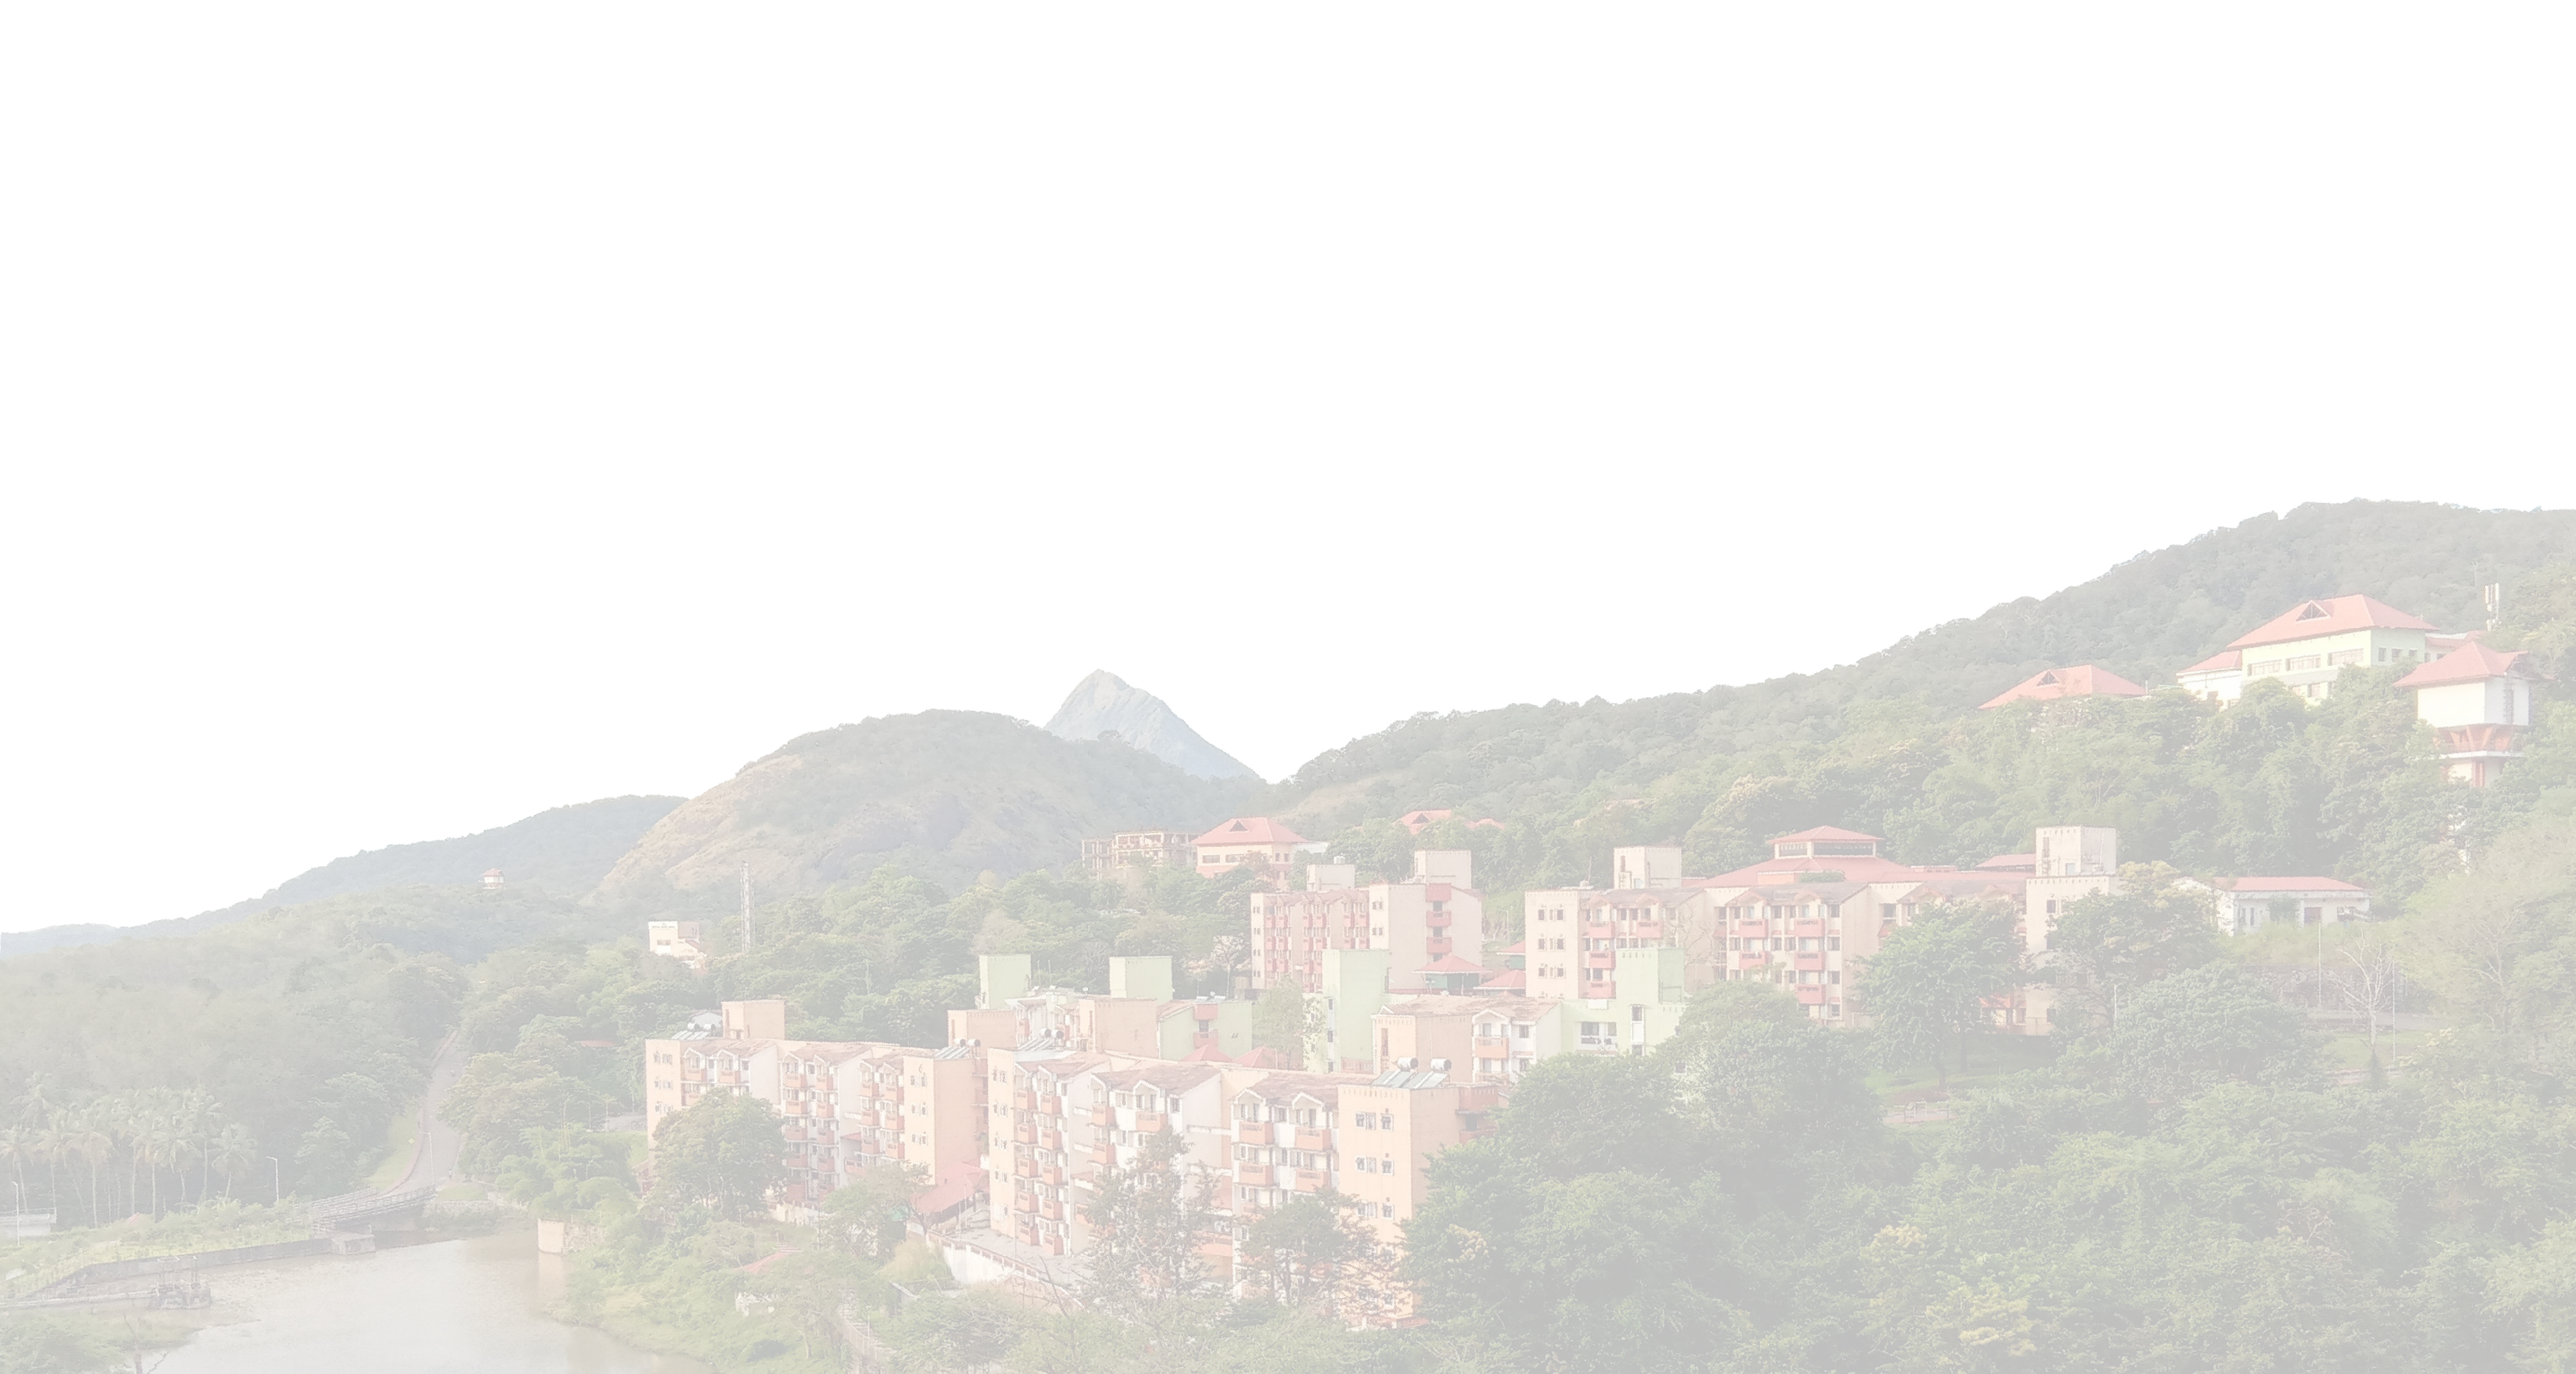
\includegraphics[width=\paperwidth,height=\paperheight]{Images/IISER_Campus_BG.png}}

\begin{frame}
  \titlepage
\end{frame}
% }


% Sections
\section{Introduction to Saturnin}
\subsection{Saturnin Basics}

\begin{frame}{Saturnin Cipher Basics}
\begin{itemize}
    \item \textbf{Saturnin} is a symmetric \alert{block cipher} designed with post-quantum security and lightweightness in mind.
    \item Key features:
    \begin{itemize}
        \item \textbf{256-bit state} and \textbf{256-bit key}.
        \item Lightweight design suitable implemented using bitsliced operations.
        \item Structured similarly to AES, but uses a 3D 4x4x4 \alert{nibble cube} state.
    \end{itemize}
    \end{itemize}

\end{frame}


\subsection{Post Quantum Motivation}
\begin{frame}{Why Post-Quantum Ciphers?}
\begin{itemize}
    \item Quantum algorithms such as \textbf{Shor's algorithm} threaten asymmetric schemes (RSA, ECC).
    \item Symmetric ciphers are more resistant, but:
    \begin{itemize}
        \item Grover's algorithm reduces brute-force cost from $2^n$ to $2^{n/2}$.
        \item Hence, to maintain $\sim 2^{128}$ security, block ciphers need \textbf{at least 256-bit keys/states}.
    \end{itemize}
    \item Research into \alert{lightweight, quantum-safe symmetric ciphers} is therefore ongoing.
\end{itemize}
\end{frame}

\subsection{Why the name Saturnin?}
\begin{frame}{Why the name Saturnin?}
    Saturnin the Duck. The duck is undeniably a symbol of lightness because it floats. It has been famously used as the reference for lightness throughout the ages. Saturnin the duck is the most famous duck in France.
    \\
    Kepler found the distance between the five known planets to be calculated by inscribing each Platonic solid inside a sphere. And saturn got associated with the cube.
    \begin{center}  \includegraphics[width=0.55\textwidth,height=0.6\textheight,keepaspectratio]{Images/Figures/duck.png}
    \includegraphics[width=0.55\textwidth,height=0.6\textheight,keepaspectratio]{Images/Figures/kepler.png}
    \includegraphics[width=0.55\textwidth,height=0.6\textheight,keepaspectratio]{Images/Figures/novel.jpg}
    \end{center}
\end{frame}




\section{Saturnin}
\subsection{Saturnin State structure}

\begin{frame}{Saturnin block and register state}
    \begin{center}
        \includegraphics[width=0.85\textwidth,height=0.9\textheight,keepaspectratio]{Images/Figures/1.jpg}
    \end{center}

\end{frame}

\begin{frame}{Terms and Definitions}

\begin{itemize}
    \item Slice: putting the z axis constant
    \item Sheet: putting the x axis constant
    \item Column: putting the x and z as constant
\end{itemize}

\begin{center}
    \includegraphics[width=0.85\textwidth,height=0.9\textheight,keepaspectratio]{Images/Figures/2.png}
\end{center}
\end{frame}

\subsection{One round of Saturnin}

\begin{frame}{Sbox}

\begin{center}
\includegraphics[width=0.9\textwidth,height=0.9\textheight,keepaspectratio]{Images/Figures/sbox.png}
\end{center}

% \begin{itemize}
%     \item SR$_r$ and SR$_r^{-1}$ sandwich the linear layer (MC) for strong diffusion.
%     \item Subkey addition only happens in odd rounds $\rightarrow$ defines a \textbf{super-round}.
% \end{itemize}

\end{frame}

\begin{frame}{Permutation}

    \begin{center}
\includegraphics[width=0.9\textwidth,height=0.9\textheight,keepaspectratio]{Images/Figures/2.png}
\end{center}
\end{frame}

\begin{frame}{Permutation}
        \begin{center}
\includegraphics[width=0.9\textwidth,height=0.9\textheight,keepaspectratio]{Images/Figures/p1.png}
\includegraphics[width=0.9\textwidth,height=0.9\textheight,keepaspectratio]{Images/Figures/p2.png}
\end{center}
\end{frame}

\begin{frame}{Permutation}
        \begin{center}
\includegraphics[width=0.9\textwidth,height=0.9\textheight,keepaspectratio]{Images/Figures/p1.png}
\includegraphics[width=0.9\textwidth,height=0.9\textheight,keepaspectratio]{Images/Figures/p3.png}
\end{center}
\end{frame}

\begin{frame}{Mixed Columns}
            \begin{center}
\includegraphics[width=0.7\textwidth,height=0.6\textheight,keepaspectratio]{Images/Figures/mc1.png}
\includegraphics[width=0.45\textwidth,height=0.5\textheight,keepaspectratio]{Images/Figures/mc2.png}
\end{center}
\end{frame}

\begin{frame}{Round function of Saturnin}

\begin{itemize}
    \item One super-round is defined as two round 2r and 2r+1
    \item Each round consists of the following transformations:
    \begin{enumerate}
        \item \textbf{S-box layer (S):} Apply $\sigma_0$ to even-index nibbles and $\sigma_1$ to odd-index nibbles.
        \item \textbf{Permutation (SR$_r$):} 
        \begin{itemize}
            \item Even rounds: Identity
            \item Odd rounds, $r \bmod 4 = 1$: SR$_{\text{slice}}$ (mixes inside slices)
            \item Odd rounds, $r \bmod 4 = 3$: SR$_{\text{sheet}}$ (mixes inside sheets)
        \end{itemize}
        \item \textbf{Linear layer (MC):} Apply 4x4 MDS matrix on each column.
        \item \textbf{Inverse permutation (SR$_r^{-1}$):} Undo the SR$_r$ applied earlier.
        \item \textbf{Subkey addition:} At the end of each super-round (odd rounds), XOR with round key + round constant.
    \end{enumerate}
\end{itemize}

\end{frame}

\section{Security}
\begin{frame}{Saturnin Security}
    \begin{itemize}
        \item Security wise: 1 super round of Saturnin = 1 round of AES
        \item Therefore, the number of rounds is 20 or 2*10(AES)
    \end{itemize}
\end{frame}


\section{Implementation}

\begin{frame}{State Representation}
    \begin{itemize}
        \item State = 256 bits, represented as 16 words of 16 bits.
        \item Arranged as a $4 \times 4$ matrix:
        \[
        \begin{bmatrix}
        x_0 & x_1 & x_2 & x_3 \\
        x_4 & x_5 & x_6 & x_7 \\
        x_8 & x_9 & x_{10} & x_{11} \\
        x_{12} & x_{13} & x_{14} & x_{15}
        \end{bmatrix}
        \]
        \item Round functions operate on this structure.
    \end{itemize}
    \end{frame}

        \begin{frame}[fragile]{ShiftRow}
            \begin{itemize}
                \item Alternate between two permutations:
                \begin{itemize}
                    \item \textbf{ShiftRowSheet (even rounds)}
                    \item \textbf{ShiftRowSlice (odd rounds)}
                \end{itemize}
            \end{itemize}
            \begin{verbatim}
            rotate_left(&s[4], 1);
            rotate_left(&s[8], 2);
            rotate_left(&s[12], 3);
            \end{verbatim}
            \end{frame}

\begin{frame}{MDS Diffusion Layer}
    \begin{itemize}
        \item State split into 4 groups: A, B, C, D.
        \item Operation sequence:
        \begin{enumerate}
            \item $C \gets C \oplus D$
            \item $A \gets A \oplus B$
            \item Apply MUL rotation on $B$ and $D$.
            \item Cross XOR again: $B \gets B \oplus C$, $D \gets D \oplus A$.
            \item Apply MUL twice on $A$ and $C$.
        \end{enumerate}
        \item Guarantees \textbf{maximum diffusion} (MDS property).
    \end{itemize}
    \end{frame}
            

    \begin{frame}[fragile]{Round Constants}
        \begin{itemize}
            \item Two constants RC0, RC1 added each round.
            \item Generated using an 8-bit LFSR.
            \item Breaks symmetry and prevents slide attacks.
        \end{itemize}
        
        \begin{verbatim}
        
        static uint8_t lfsr(uint8_t x) {
            return (x << 1) ^ (0x1B & -(x >> 7));
        }
        
        // each round
        RC0 = lfsr(RC0);
        RC1 = lfsr(RC1);
        state[0] ^= RC0;
        state[4] ^= RC1;
    \end{verbatim}
        \end{frame}
\section{Impossible Differential Trail on Saturnin}
\begin{frame}{Two impossible Differential Trails}
    \begin{center}
        \includegraphics[width=0.85\textwidth,height=0.9\textheight,keepaspectratio]{Images/Figures/imp_diff.png}
    \end{center}
\end{frame}

\begin{frame}{Differential Trail 1}
    \begin{itemize}
        \item Its a 4 round Impossible Differential, meeting in the middle.
        \item Starts with a small number of active nibbles in the state.
        \item We start from the left from the top and the MD step which has SR slice diffuses the sboxes only in the slice
        \item Hence when we start from the bottom, the trail doesnt match with each other.
        \item So the first round starts from even then $x\%4 = 1$ so 4 5 6 7, becuase we are using SR slice.
        \end{itemize}
    \end{frame}
    
    \begin{frame}{Differential Trail 2}
        \begin{itemize}
            \item Starts with a small number of active nibbles in the state.
            \item We start from the left from the top and here the MS step diffuses differences across sheets.
            \item When traced from the bottom, the activity propagates differently — this time the trail aligns better due to stronger diffusion.
            \item So the first round starts from even then $x\%4 = 3$ so 2 3 4 5, because we are using SR sheet.
        \end{itemize}
    \end{frame}
    
    
\input{Sections/Summing Up}


% % References
% \begin{frame}[allowframebreaks]
%     \frametitle{References}
%     \nocite{*}
%     \printbibliography
% \end{frame}

% % Appendix
% \appendix
% \input{Sections/6_Appendix}

\end{document}
